
\documentclass{beamer}
\usetheme{ucl}

\usepackage[utf8]{inputenc}


%%% Increase the height of the banner: the argument is a scale factor >=1.0
%\setbeamertemplate{banner}[ucl][10.0]

%%% Change the colour of the main banner
%%% The background should be one of the UCL colours (except pink or white):
%%%   black,darkpurple,darkred,darkblue,darkgreen,darkbrown,richred,midred,
%%%   navyblue,midgreen,darkgrey,orange,brightblue,brightgreen,lightgrey,
%%%   lightpurple,yellow,lightblue,lightgreen,stone
\setbeamercolor{banner}{bg=darkpurple}
%\setbeamercolor{banner}{bg=yellow,fg=black}

%%% Add a stripe behind the banner
%\setbeamercolor{banner stripe}{bg=darkpurple,fg=black}

%%% The main structural elements
\setbeamercolor{structure}{fg=black}

%%% Author/Title/Date and slide number in the footline
\setbeamertemplate{footline}[author title date]

%%% Puts the section/subsection in the headline
% \setbeamertemplate{headline}[section]

%%% Puts a navigation bar on top of the banner
%%% For this to work correctly, the each \section command needs to be
%%% followed by a \subsection. Requires one extra compile.
% \setbeamertemplate{headline}[miniframes]
%%% Accepts an optional argument determining the width
% \setbeamertemplate{headline}[miniframes][0.3\paperwidth]


%%% Puts the frame title in the banner
%%% Won't work correctly with the above headline templates
%\useoutertheme{ucltitlebanner}
%%% Similar to above, but smaller (and puts subtitle on same line as title)
\useoutertheme[small]{ucltitlebanner}

%%% Gives block elements (theorems, examples) a border
% \useinnertheme{blockborder}
%%% Sets the body of block elements to be clear
% \setbeamercolor{block body}{bg=white,fg=black}

%%% Include CSML logo on title slide
%\titlegraphic{\includegraphics[width=0.16\paperwidth]{csml_logo}}

%%% Include CSML logo in bottom right corner of all slides
%\logo{\includegraphics[width=0.12\paperwidth]{csml_logo}}

%%% Set a background colour
% \setbeamercolor{background canvas}{bg=lightgrey}

%%% Set a background image
%%% Some sample images are available from the UCL image store:
%%%   https://www.imagestore.ucl.ac.uk/home/start
% \setbeamertemplate{background canvas}{%
%   \includegraphics[width=\paperwidth]{imagename}}



%%%%%% Some other settings that can make things look nicer
%%% Set a smaller indent for description environment
\setbeamersize{description width=2em}
%%% Remove nav symbols (and shift any logo down to corner)
\setbeamertemplate{navigation symbols}{\vspace{-2ex}}








\DeclareMathOperator{\Cov}{Cov}
\DeclareMathOperator{\Var}{Var}
\DeclareMathOperator{\E}{\mathbb{E}}
\DeclareMathOperator{\Proba}{\mathbb{P}}

\newcommand{\Covb}[2]{\ensuremath{\Cov\!\left[#1,#2\right]}}
\newcommand{\Eb}[1]{\ensuremath{\E\!\left[#1\right]}}
\newcommand{\Pb}[1]{\ensuremath{\Proba\!\left[#1\right]}}
\newcommand{\Varb}[1]{\ensuremath{\Var\!\left[#1\right]}}

% norm
\newcommand{\norm}[1]{\| #1 \|}

\newcommand{\indep}{\rotatebox[origin=c]{90}{$\models$}}





\usepackage{mathptmx,amsmath,amssymb,graphicx,bibentry,bbm,ragged2e}
\usepackage[english]{babel}

\makeatletter

\newcommand{\noun}[1]{\textsc{#1}}
\newcommand{\jitem}[1]{\item \begin{justify} #1 \end{justify} \vfill{}}
\newcommand{\sframe}[2]{\frame{\frametitle{#1} #2}}

\newenvironment{centercolumns}{\begin{columns}[c]}{\end{columns}}
%\newenvironment{jitem}{\begin{justify}\begin{itemize}}{\end{itemize}\end{justify}}



%\usetheme{Warsaw}
%\setbeamertemplate{footline}[text line]{}
%\setbeamertemplate{headline}{}
%\setbeamercolor{structure}{fg=purple!50!blue, bg=purple!50!blue}

%\setbeamersize{text margin left=15pt,text margin right=15pt}

%\setbeamercovered{transparent}


\@ifundefined{showcaptionsetup}{}{%
 \PassOptionsToPackage{caption=false}{subfig}}
\usepackage{subfig}

\usepackage[utf8]{inputenc}
\usepackage[T1]{fontenc}

\usepackage{multirow}


\makeatother

\def \draft {1}

\usepackage{xparse}
\usepackage{ifthen}
\DeclareDocumentCommand{\comment}{m o o o o}
{\ifthenelse{\draft=1}{
    \textcolor{red}{\textbf{C : }#1}
    \IfValueT{#2}{\textcolor{blue}{\textbf{A1 : }#2}}
    \IfValueT{#3}{\textcolor{ForestGreen}{\textbf{A2 : }#3}}
    \IfValueT{#4}{\textcolor{red!50!blue}{\textbf{A3 : }#4}}
    \IfValueT{#5}{\textcolor{Aquamarine}{\textbf{A4 : }#5}}
 }{}
}
\newcommand{\todo}[1]{
\ifthenelse{\draft=1}{\textcolor{red!50!blue}{\textbf{TODO : \textit{#1}}}}{}
}




\begin{document}

\title
[MATSim transport modelling]{Integration of the MATSim transport model into the DAFNI platform}
\author[Raimbault]{J.~Raimbault$^{1,2,3,\ast}$\\\medskip
$^{\ast}$\texttt{j.raimbault@ucl.ac.uk}
}

\institute[UCL]{$^{1}$Center for Advanced Spatial Analysis, University College London\\
$^{2}$UPS CNRS 3611 Complex Systems Institute Paris\\
$^{3}$UMR CNRS 8504 G{\'e}ographie-cit{\'e}s
}




\date[24/03/2021]{DAFNI Roadshow - UTSG\\
24th March 2021\\
}

\frame{\maketitle}



\section{Introduction}



\sframe{Urban transportation models}{

\textit{MATSim model: heterogenous data and integration of many sub-models}

\medskip

\begin{center}
	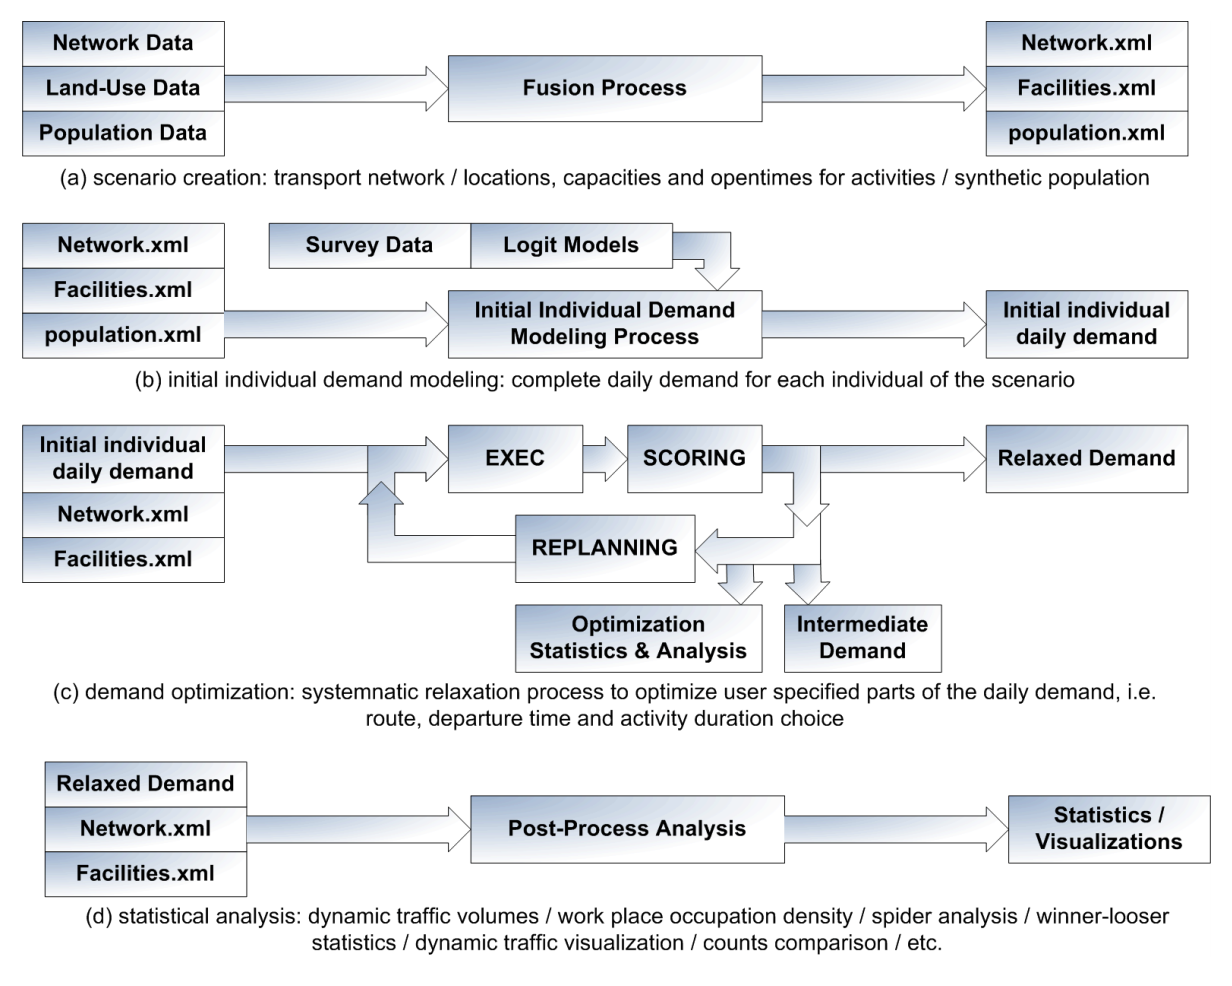
\includegraphics[height=0.7\textheight]{figures/matsim.png}	
\end{center}

Source: \cite{balmer2009matsim}

}

\sframe{Land-use transport models}{

\textit{Land-use transport models as a progressive complexification through coupling of detailed sub-models}

\medskip

\begin{center}
	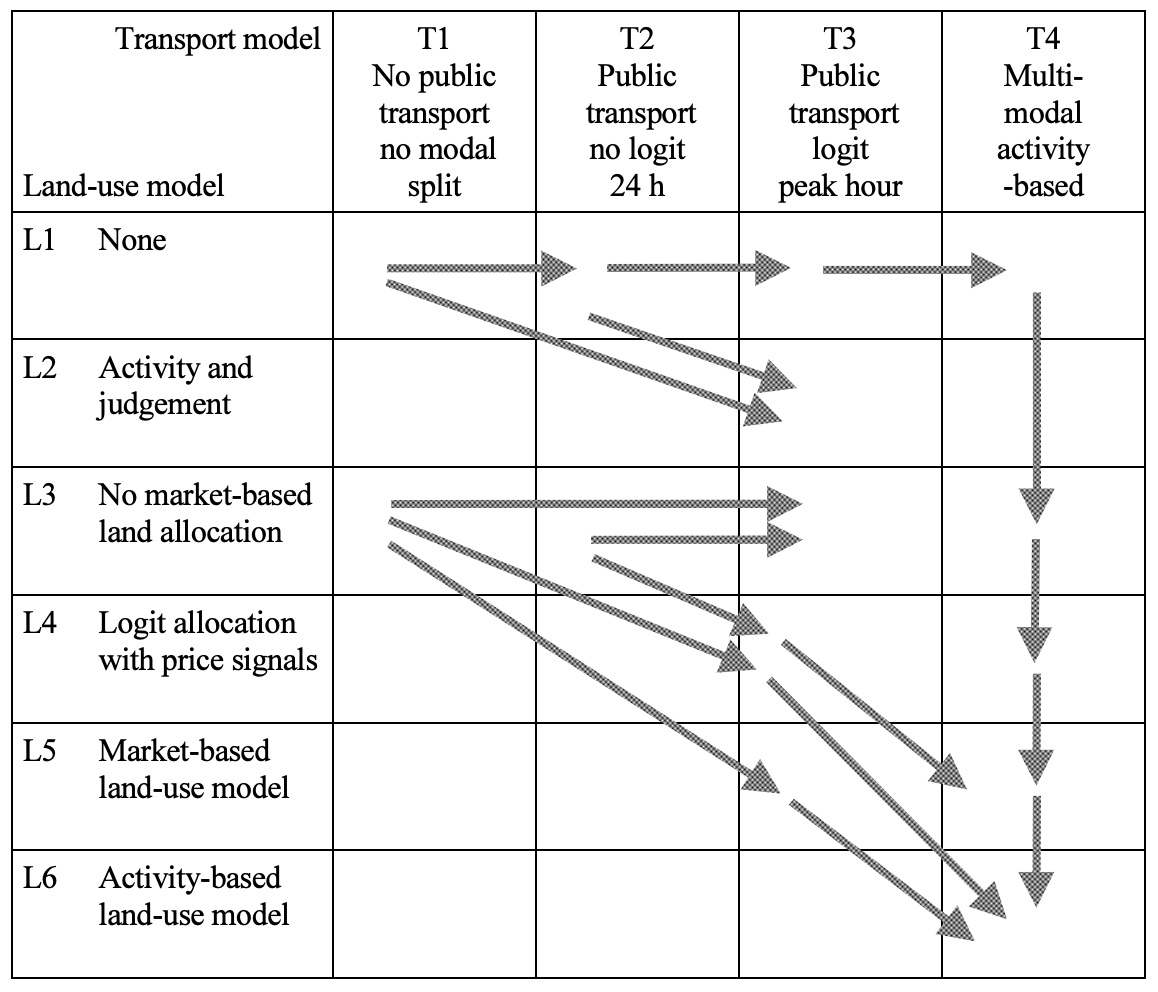
\includegraphics[width=0.45\linewidth]{figures/wegener1.png}\hspace{0.3cm}
	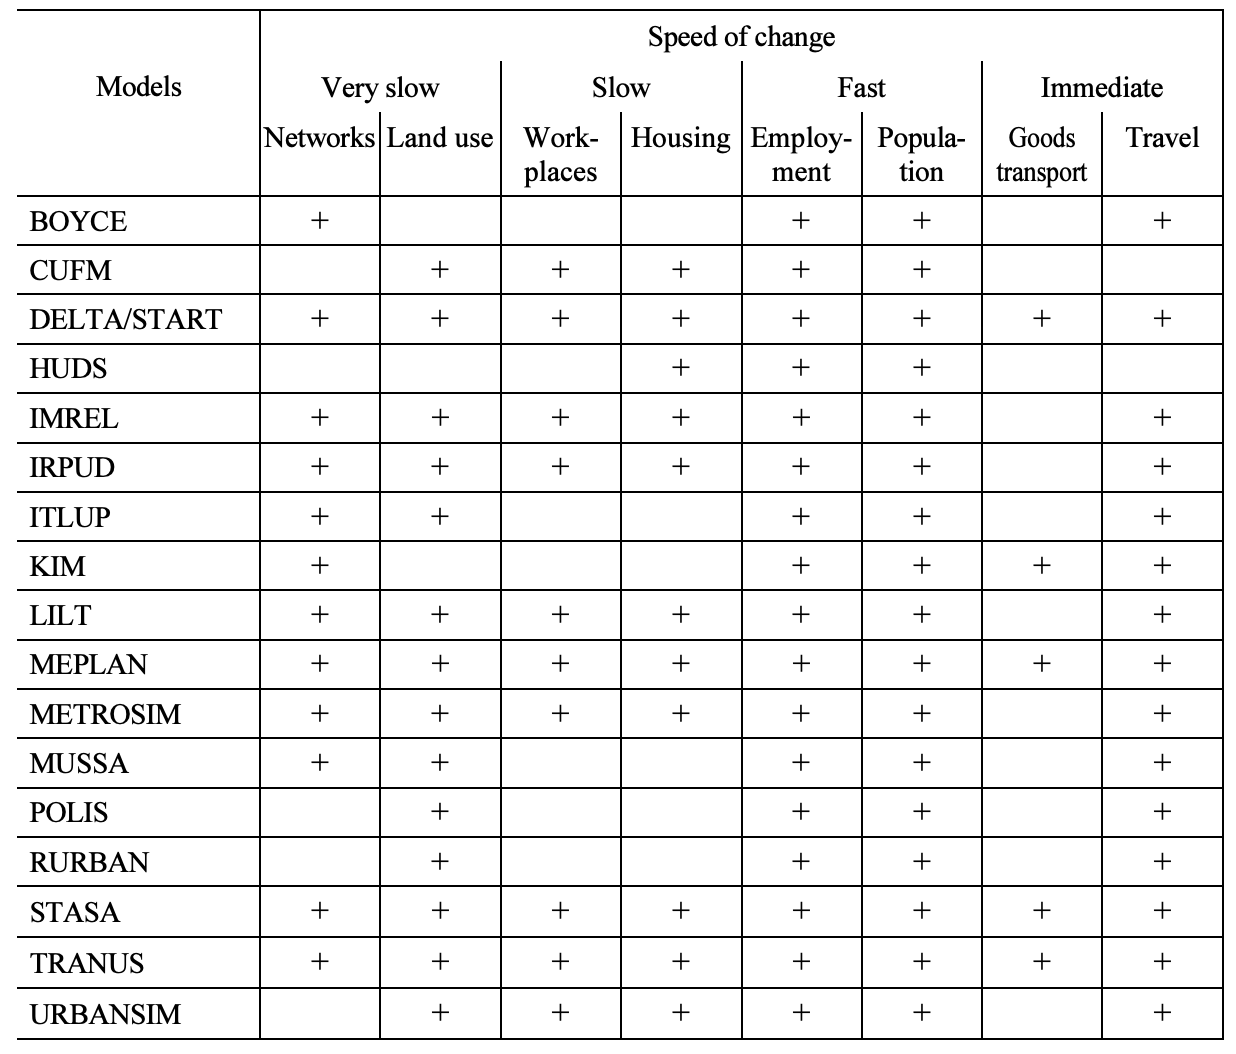
\includegraphics[width=0.45\linewidth]{figures/wegener2.png}
\end{center}

Source: \cite{wegener2004land}

}


\sframe{Towards modular models using workflow systems}{


\textit{Build modular urban transportation models from the bottom-up using scientific workflow systems, open source sub-models and open data}

\medskip

$\rightarrow$ Sub-models coupled into the workflow, can be easily replaced

$\rightarrow$ Reproducibility and transparency

$\rightarrow$ Easier transferability of model application

$\rightarrow$ Application of model validation methods

\medskip

\textbf{Implementation: } \textit{integration of the MATSim transport model into the DAFNI platform}


}


\section{Matsim}

% More particularly, we demonstrate this approach by building a modular four-step multimodal trans- portation model using only open-source projects. We couple together the MATSim model (MATSim Community) to simulate the transportation system, the SPENSER model (University of Leeds) for the generation of synthetic population, the QUANT model (University College London) to estimate spatial interactions, and the spatialdata library (OpenMOLE Community) for data preparation. The model is integrated into the DAFNI facility (https://dafni.ac.uk/) which provides a scientific work- flow system for model integration and coupling, direct access to relevant open datasets, visualisation functionalities, and access to a High Performance Computing infrastructure.


\sframe{Case study: integrated models}{



\textbf{Case study:} \textit{Construct a modular four-step multimodal transportation model using open source projects and data}

\bigskip

\textbf{Integrated models:}

\begin{itemize}
	\item MATSim model (MATSim Community) for the transportation system \url{https://www.matsim.org/} \cite{horni2016multi}
	\item SPENSER model (University of Leeds) for the synthetic population \url{https://github.com/nismod/microsimulation}
	\item QUANT model (CASA, University College London) for spatial interactions to generate home-work plans \url{http://quant.casa.ucl.ac.uk/} \cite{milton2019accelerating} (\textit{specific scala implementation})
	\item spatialdata library (OpenMOLE community) for data processing \url{https://github.com/openmole/spatialdata} \cite{raimbault2020scala}
\end{itemize}



}

\sframe{Case study: data and implementation}{


\textbf{Data:}

Generic for any Functional Urban Area (GHSL \cite{florczyk2019ghsl}) in the UK: NOMIS census, OrdnanceSurvey roads, Transport National Dataset


\medskip

\textbf{Implementation}

Currently integrated into the DAFNI platform:

\begin{itemize}
	\item synthetic SPENSER population with uniform job locations
	\item QUANT model to generate home-work commuting flows
	\item network and plans prepared into MATSim xml files and fed into a one-mode MATSim (multimodal version still tested locally)
	\item models integrated as Docker containers
\end{itemize}



}



\sframe{DAFNI workflow for coupled model}{

\centering

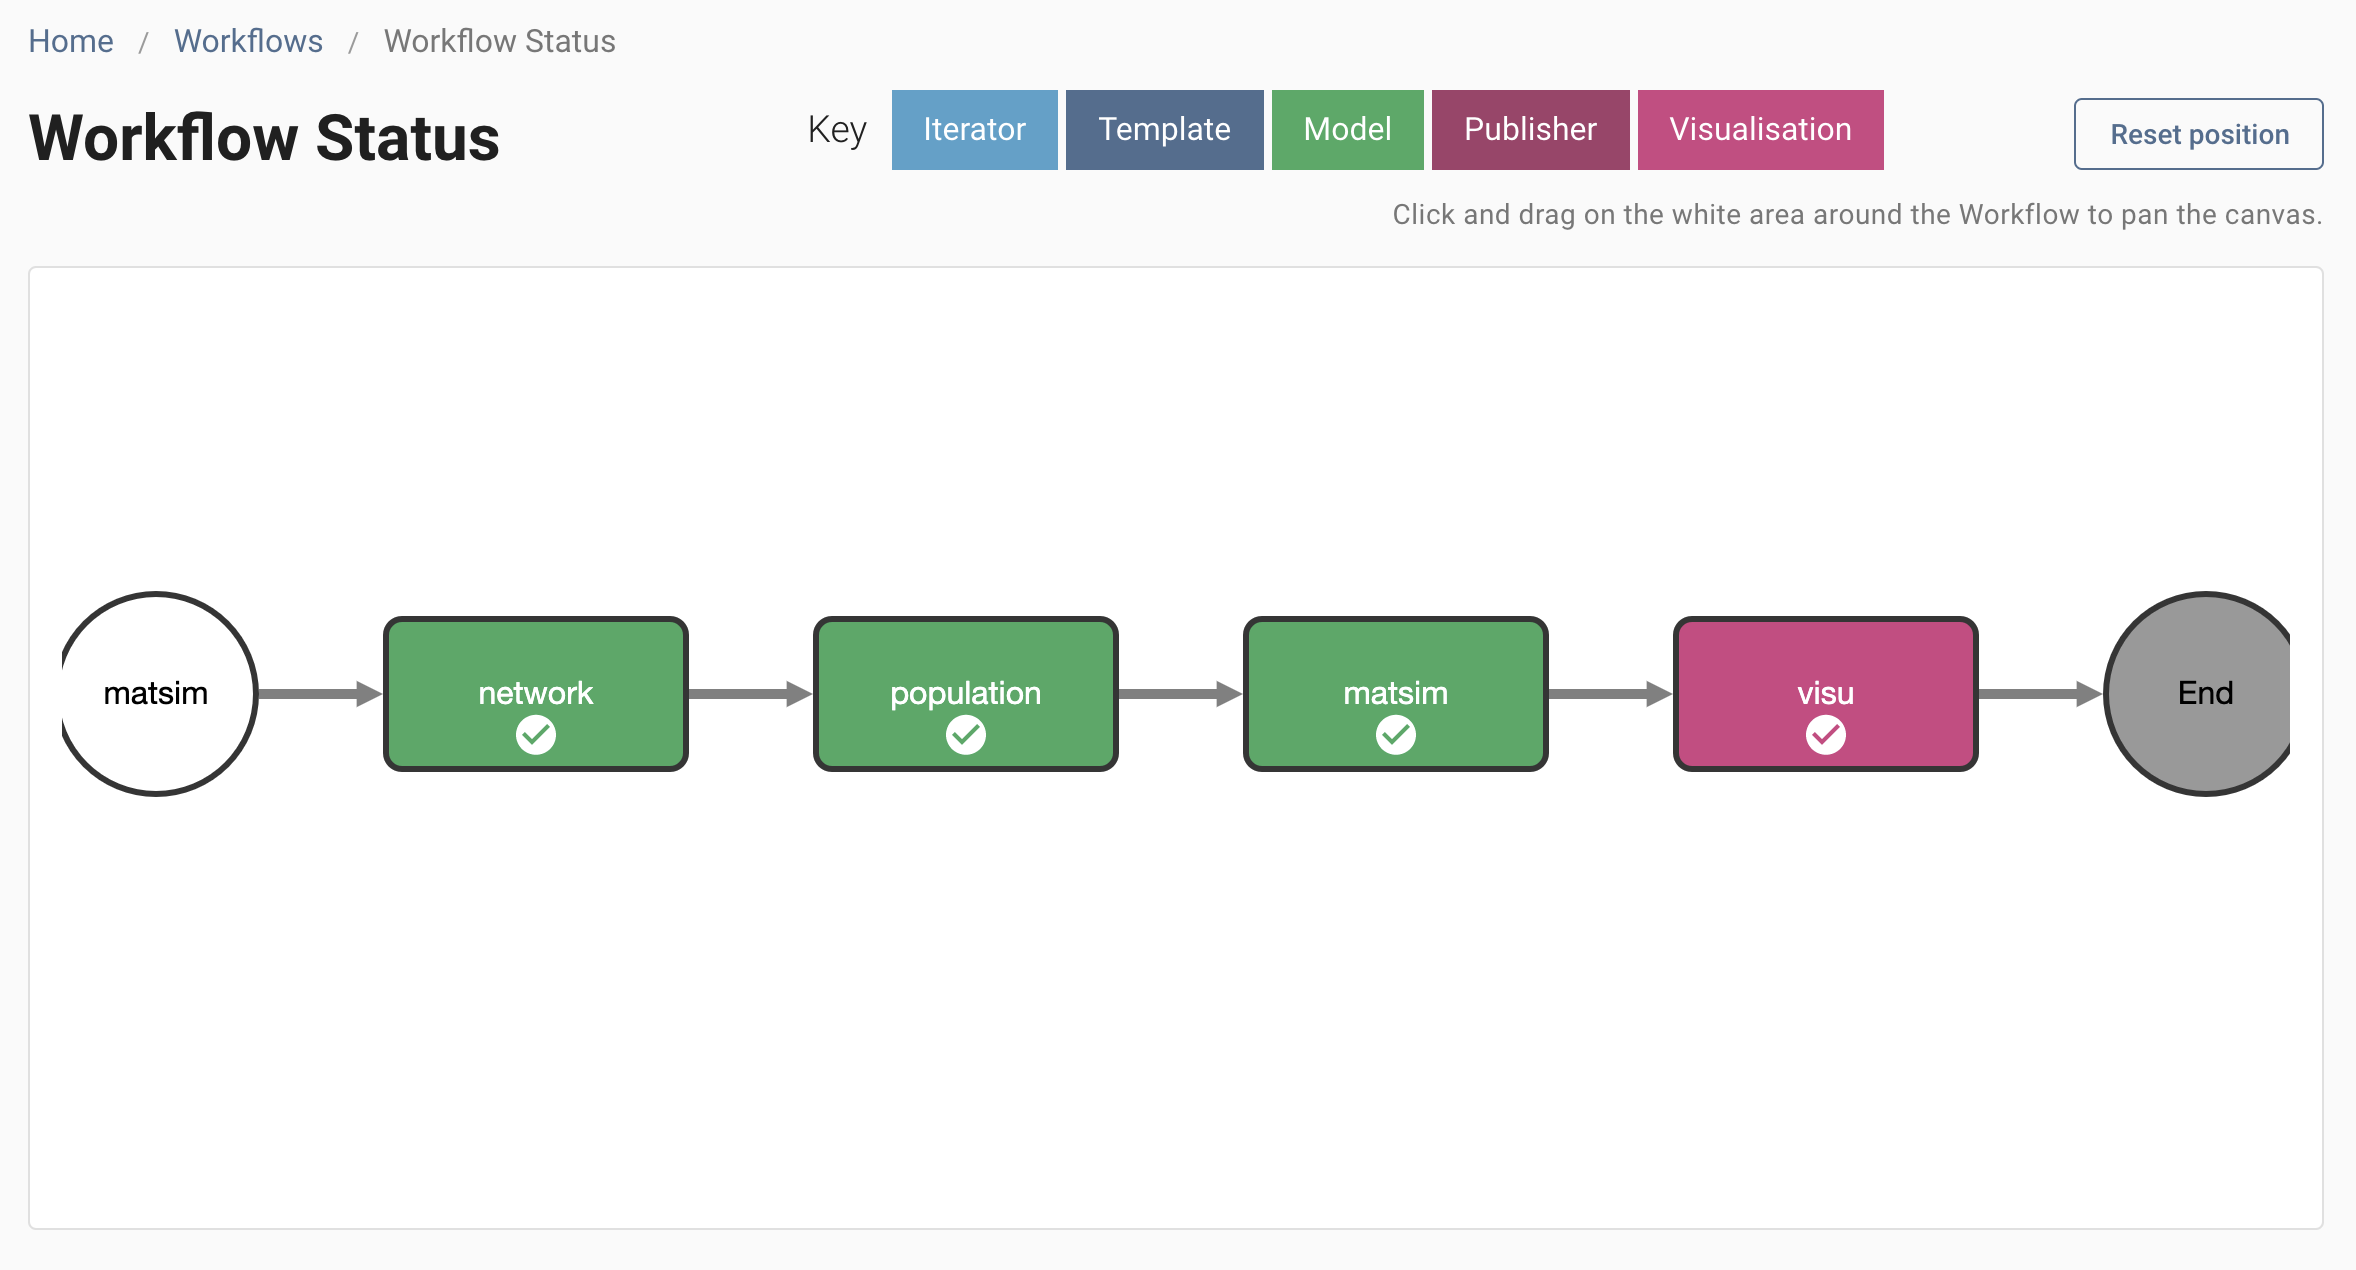
\includegraphics[width=\linewidth]{figures/matsim_workflow.png}

}


% The model is run on all functional urban areas in the UK. We show first results of numerical experiments comparing the use of the spatial interaction model with a null model to generate transport demand. We also study the role of stochasticity on model outputs, and show that spatial configuration has a significant influence.

\sframe{Visualization within DAFNI}{

\begin{center}
	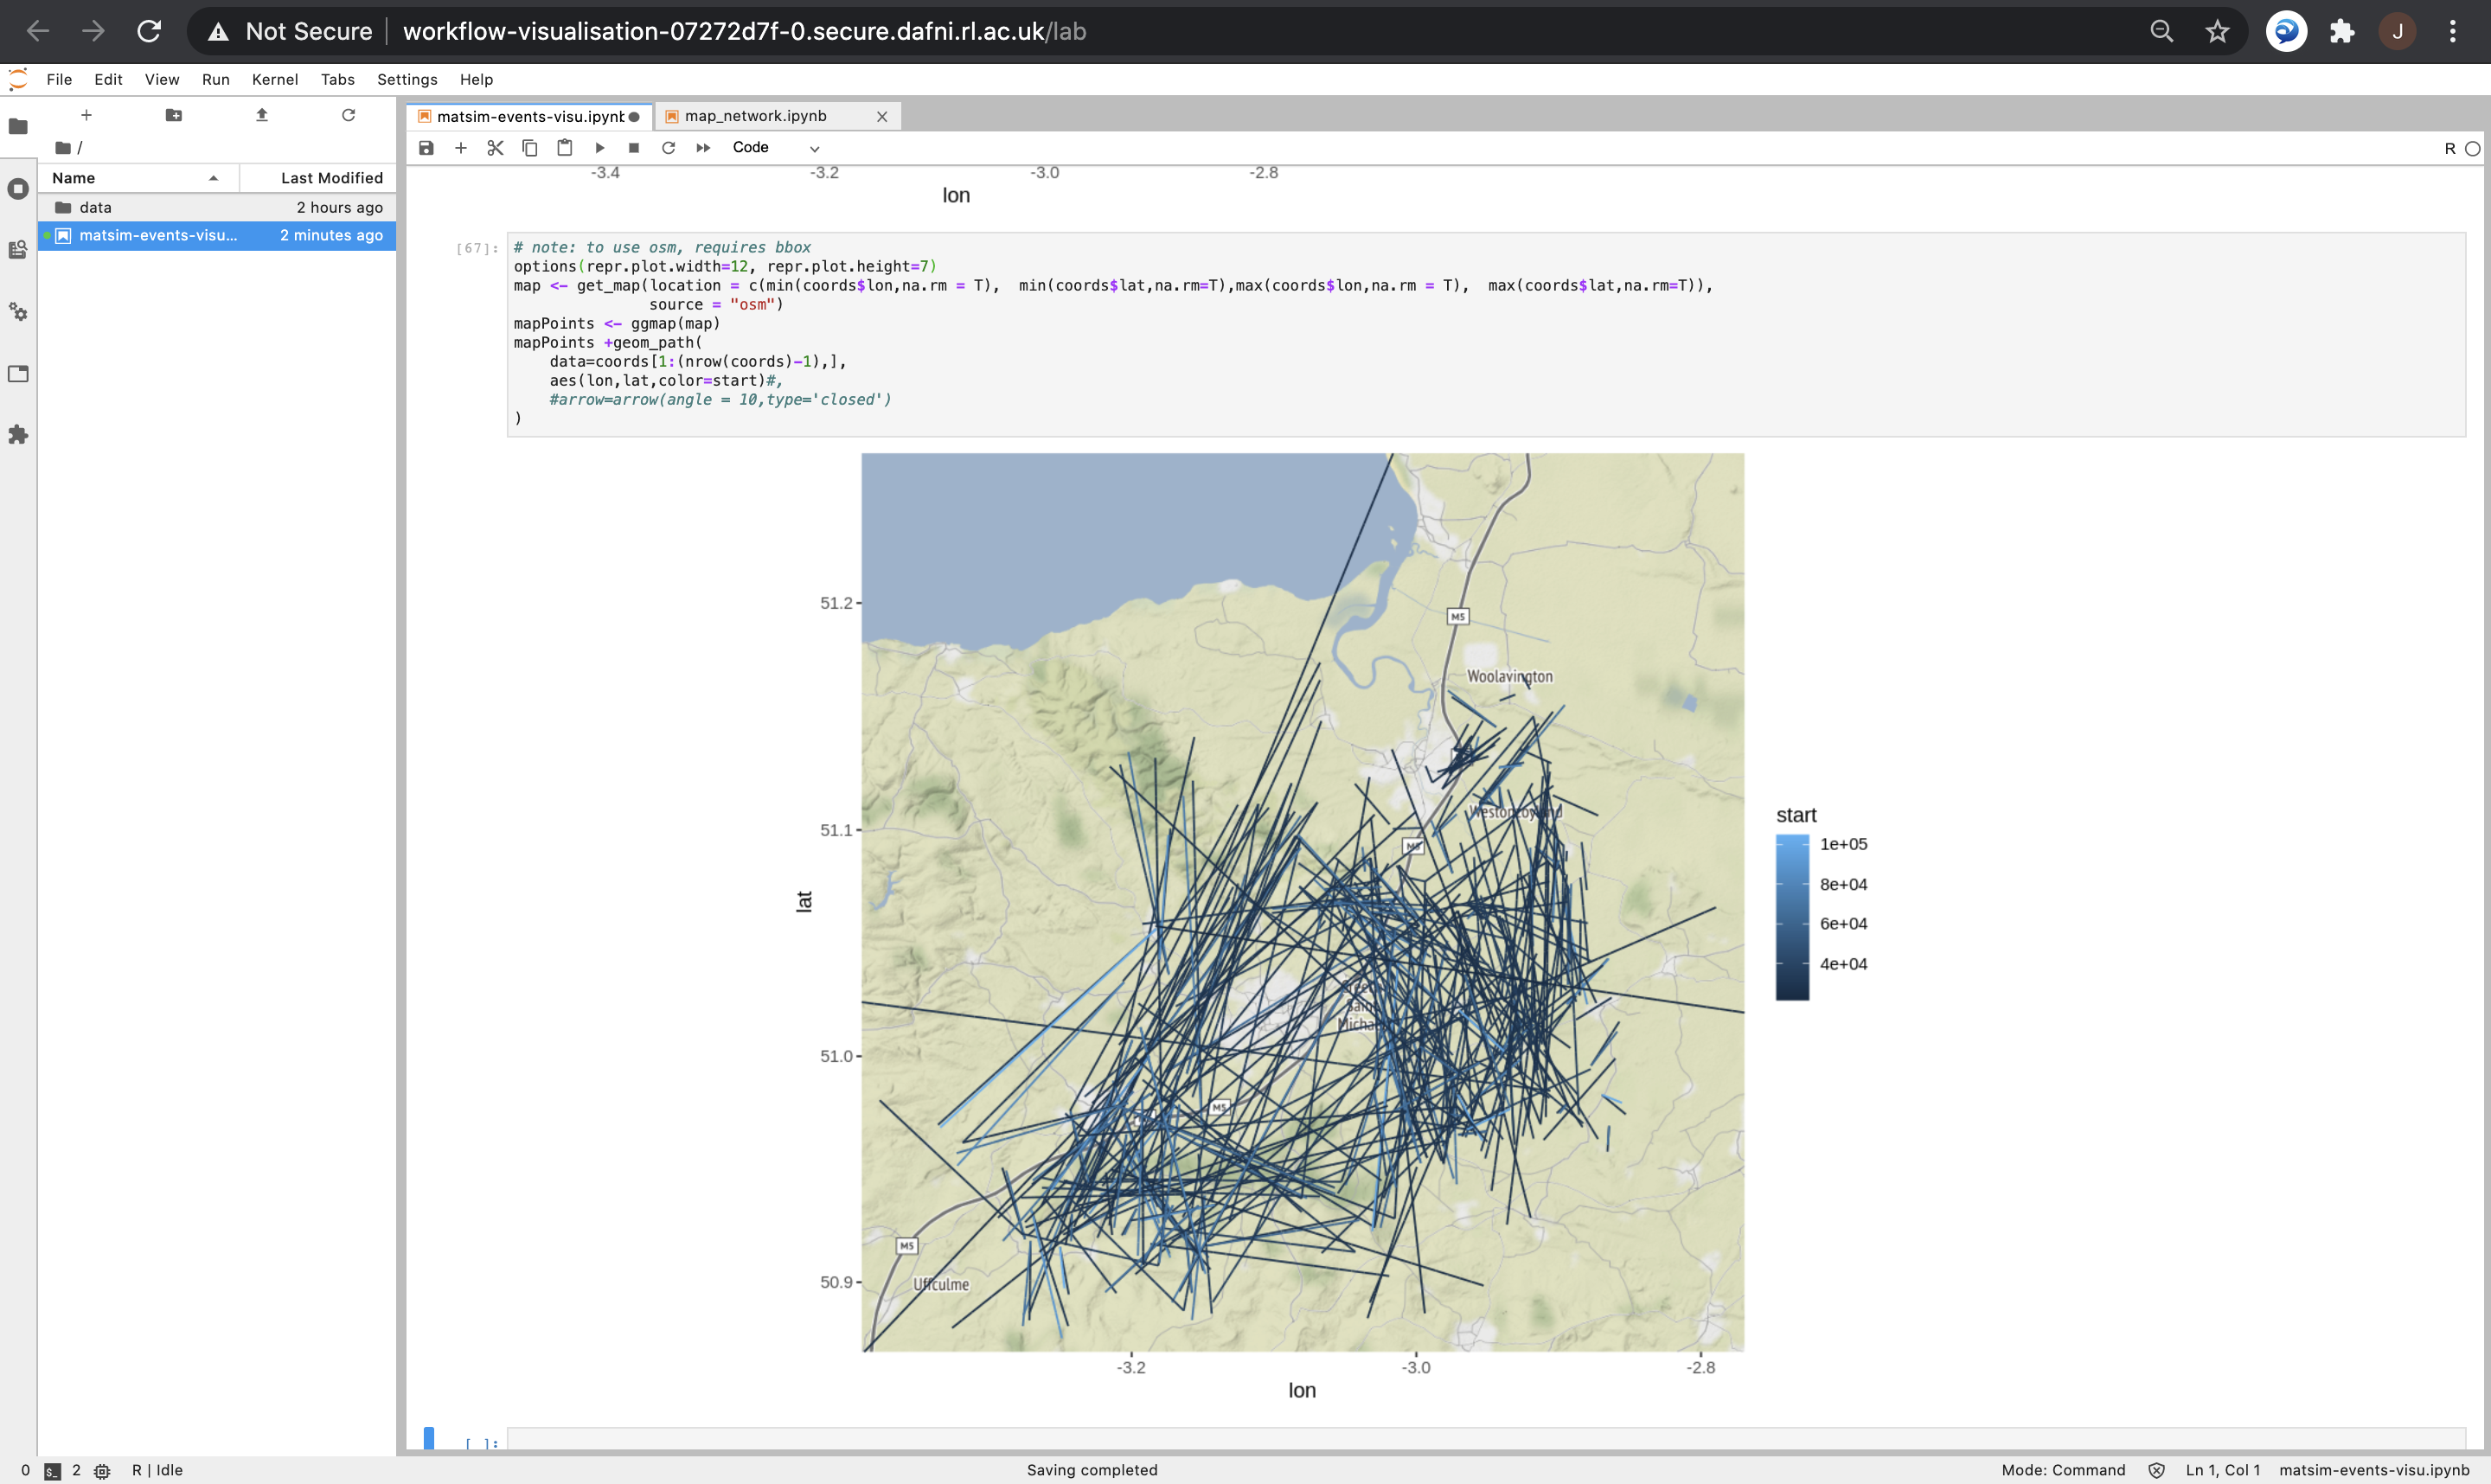
\includegraphics[width=\linewidth]{figures/visu_trips.png}	
\end{center}

}





\sframe{Simulation results: travel distances}{

% note: spatial interaction not implemented yet: simple synthetic pop
% discuss Matsim params? not needed - too complicated (reserve slide? not time! -> link to workflow)

\begin{center}
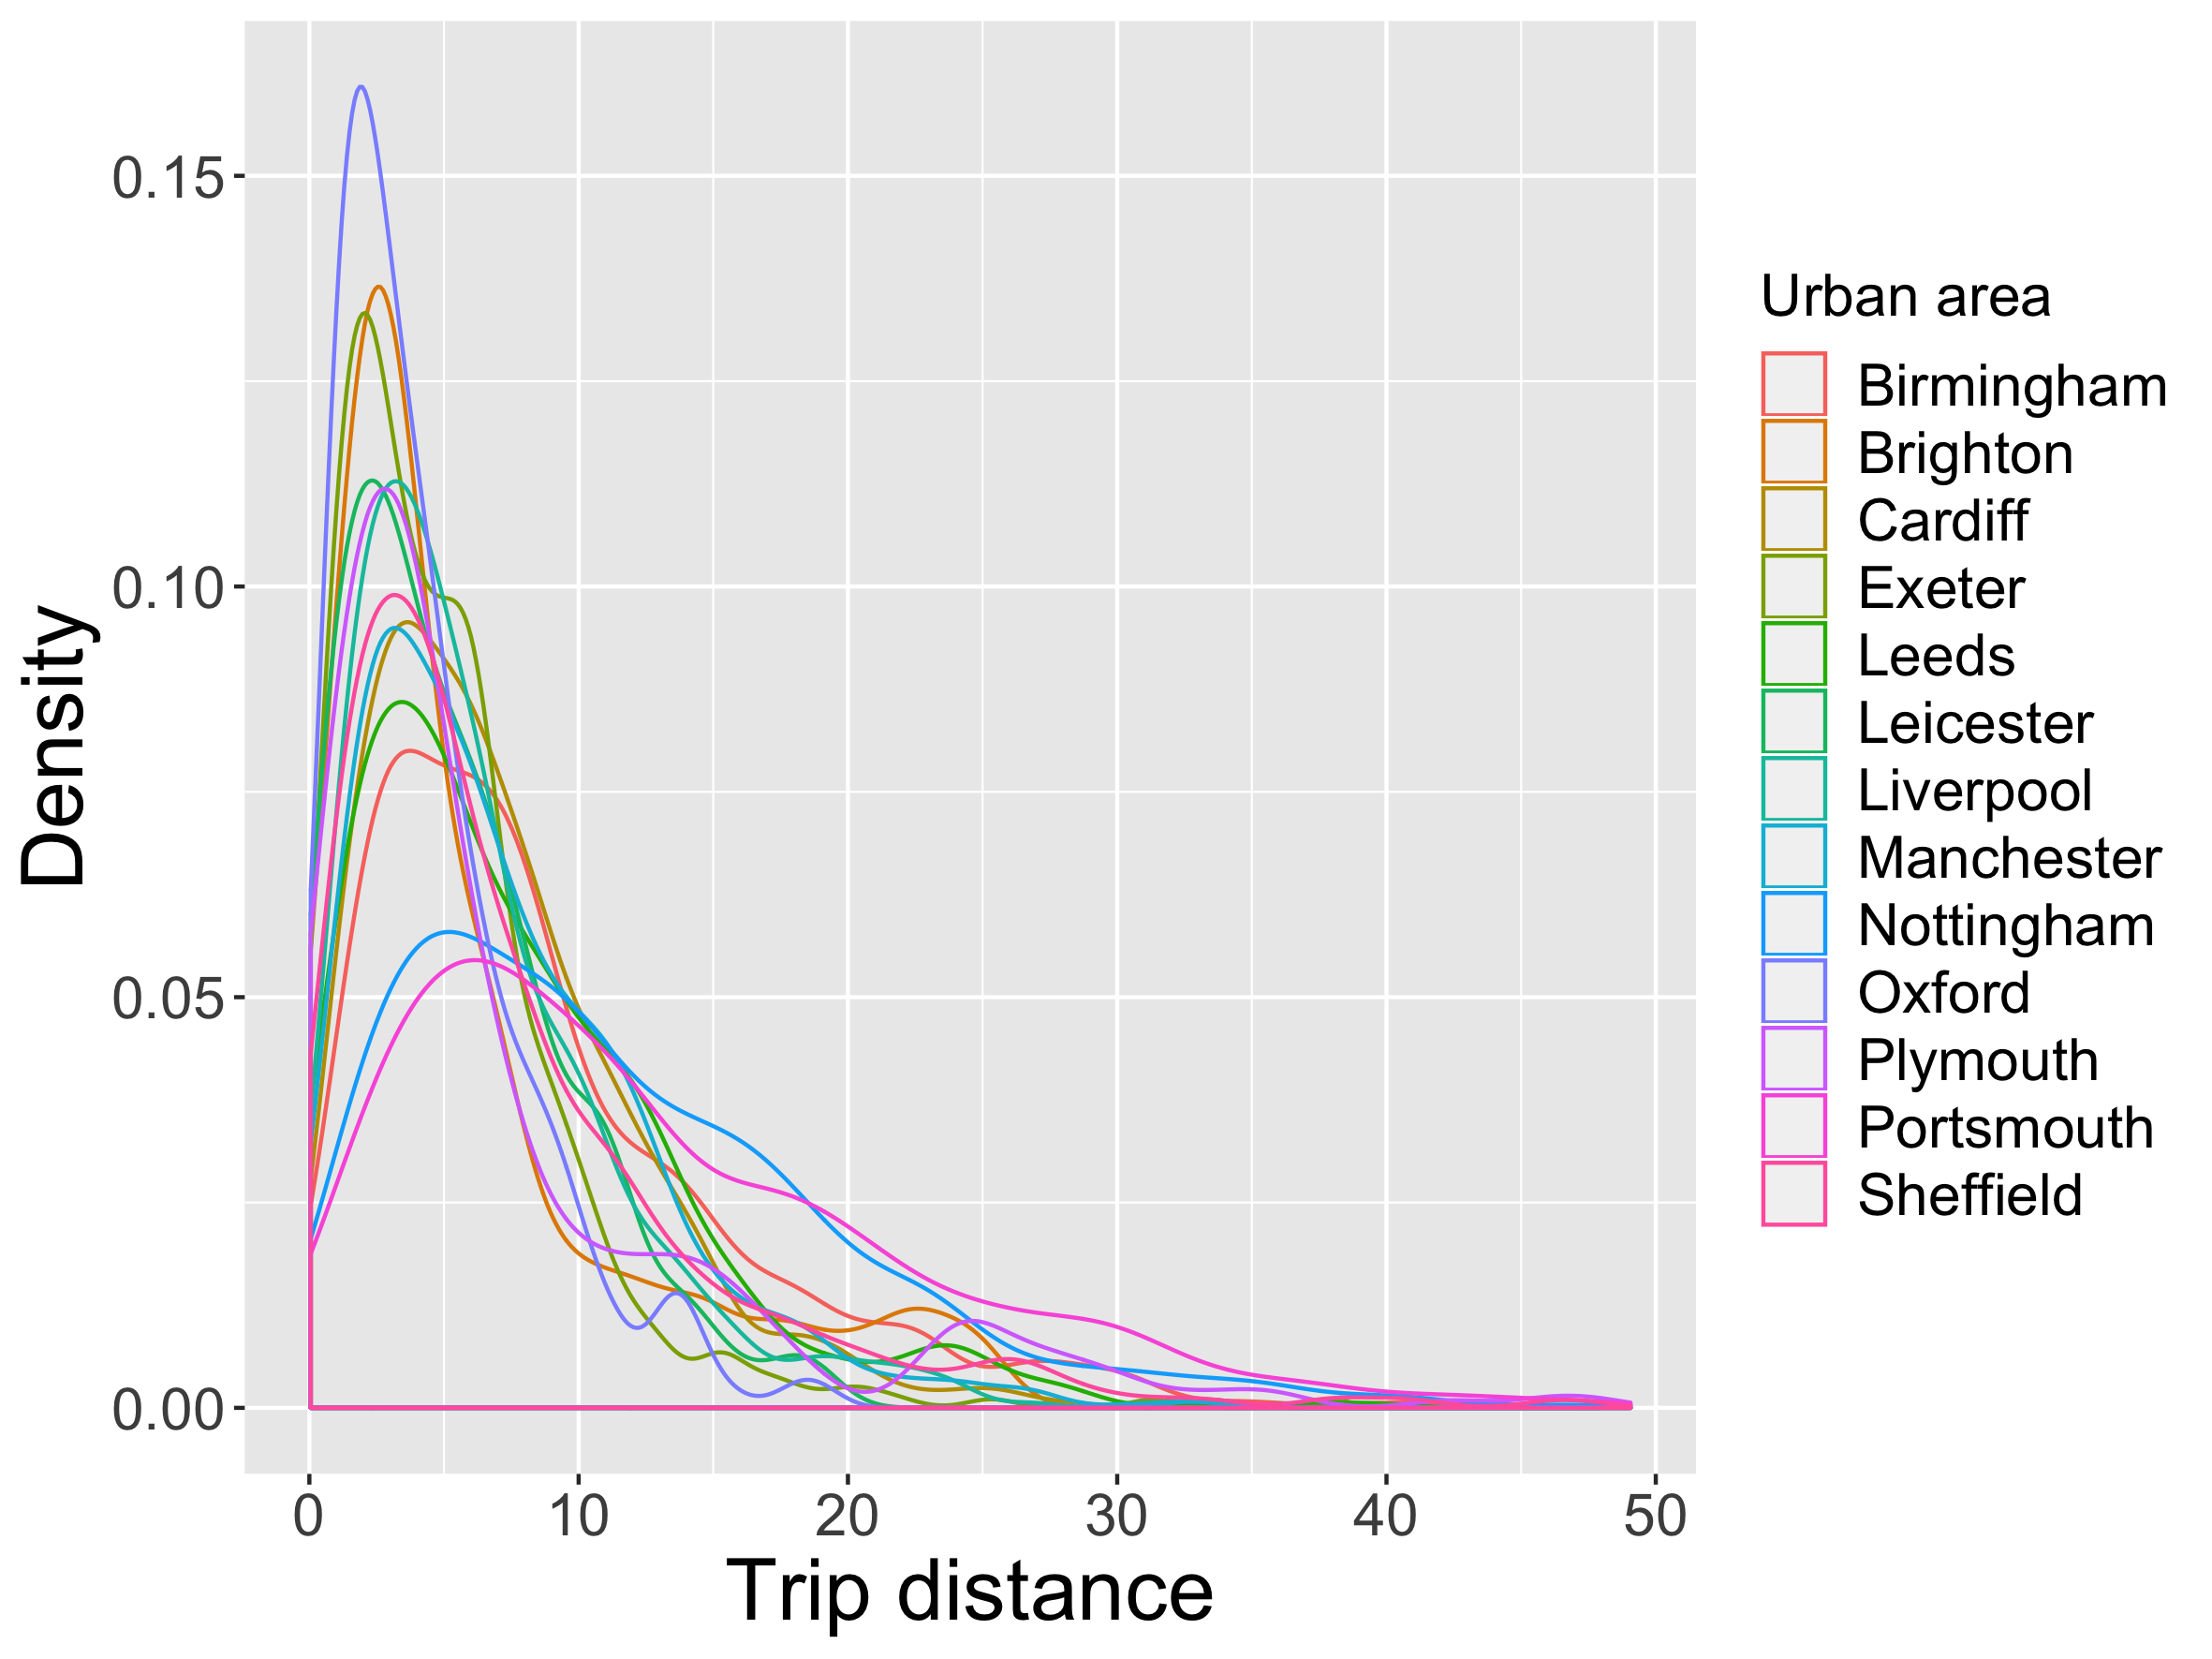
\includegraphics[width=0.9\linewidth]{figures/distances_allFUAs.png}
\end{center}

}

\sframe{Daily travel patterns}{

\begin{center}
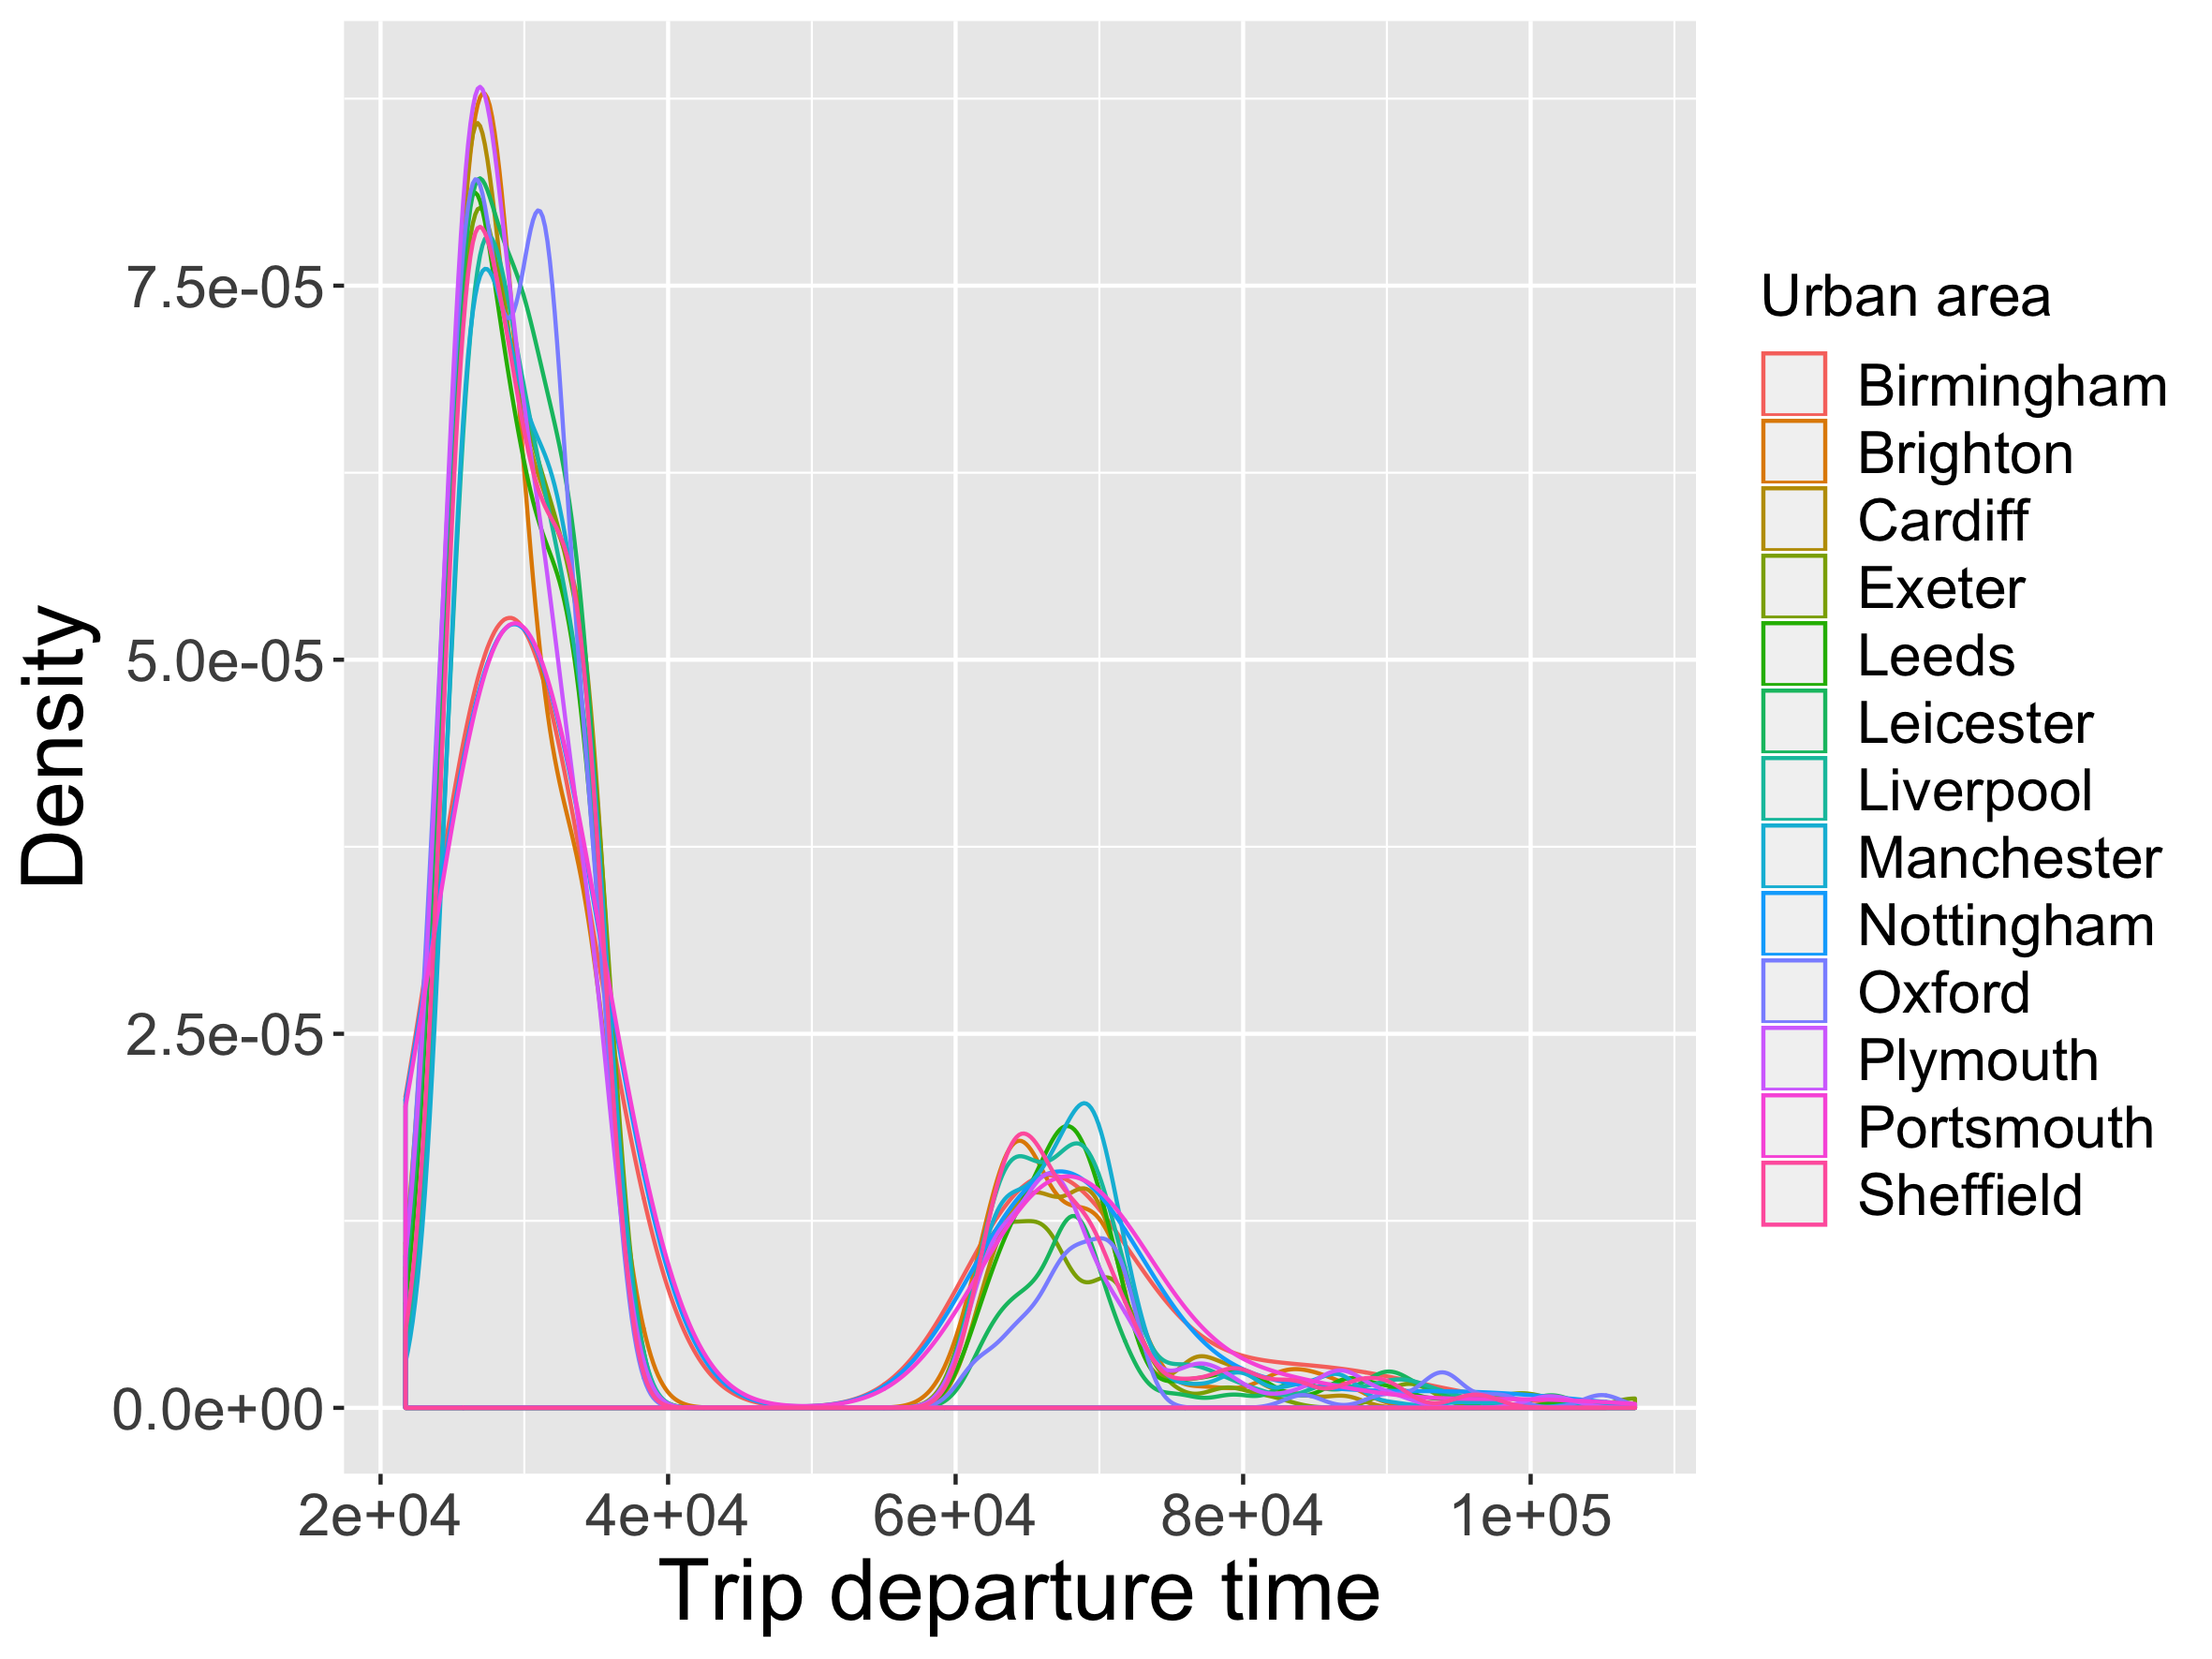
\includegraphics[width=0.9\linewidth]{figures/departuretimes_allFUAs.png}
\end{center}

}



\sframe{Role of stochasticity}{

\begin{center}
	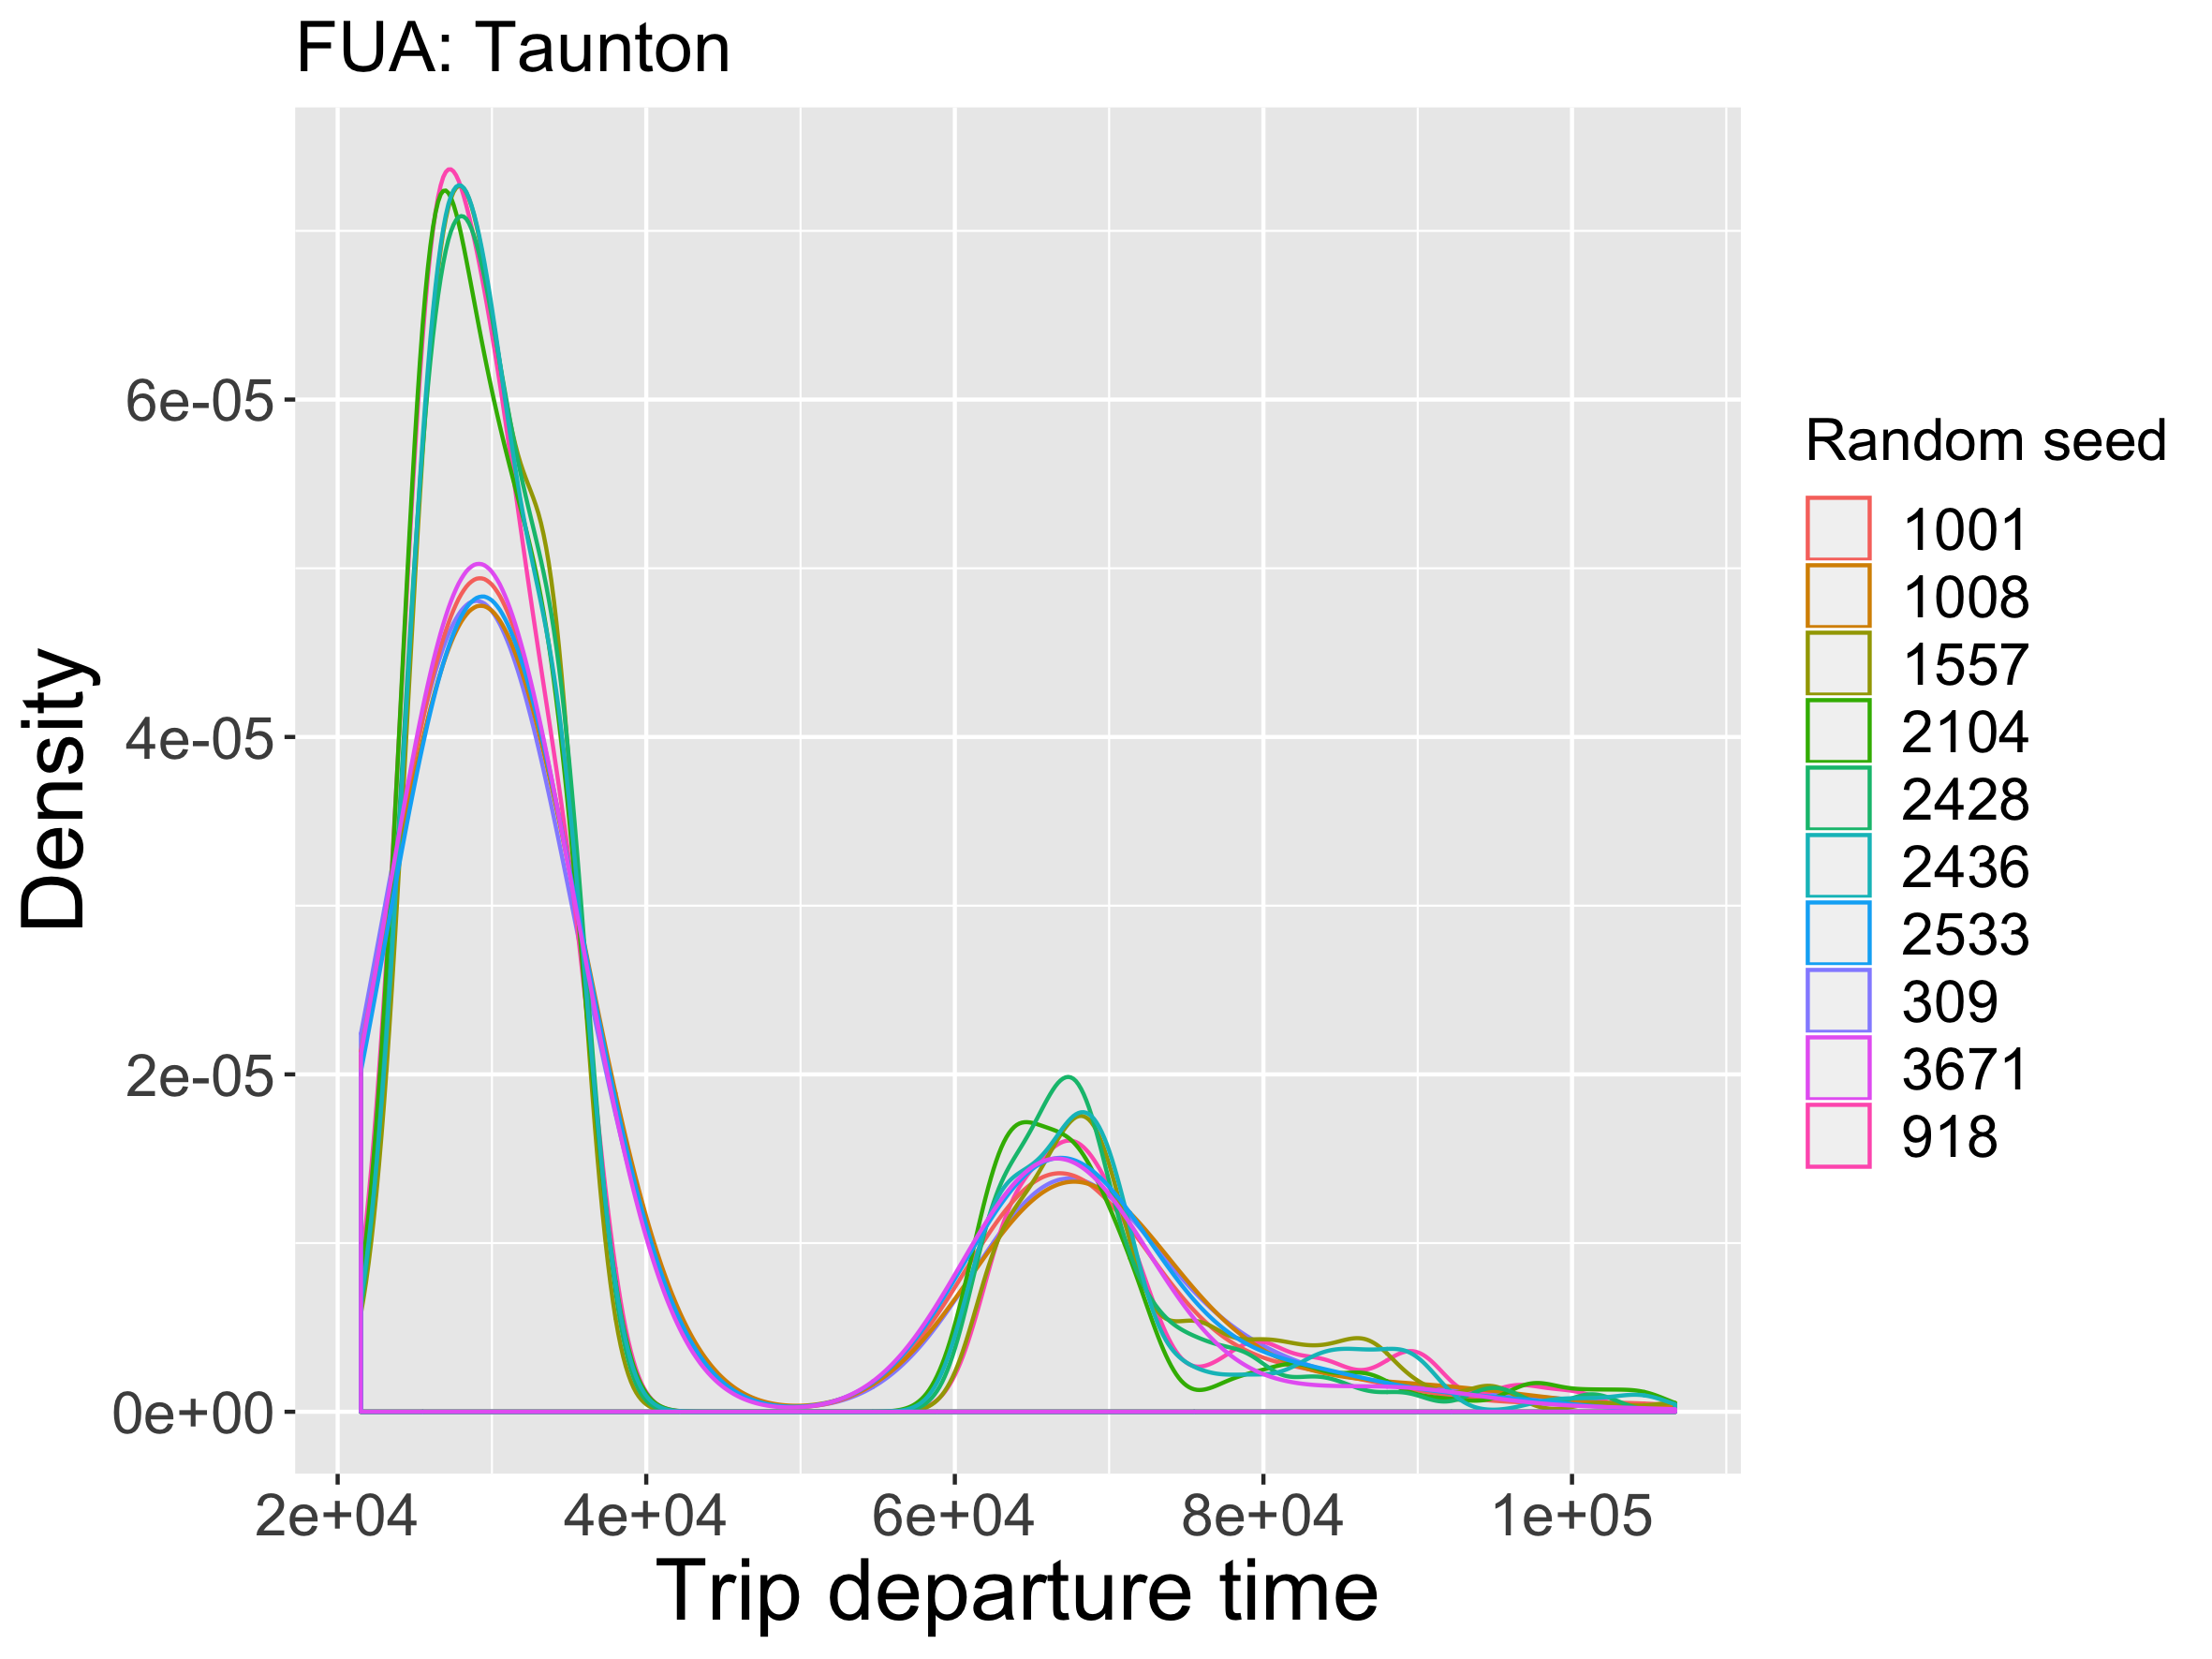
\includegraphics[width=0.9\linewidth]{figures/stochasticity_Taunton.png}	
\end{center}


}


\sframe{Validation: towards spatial sensitivity analysis}{

\centering

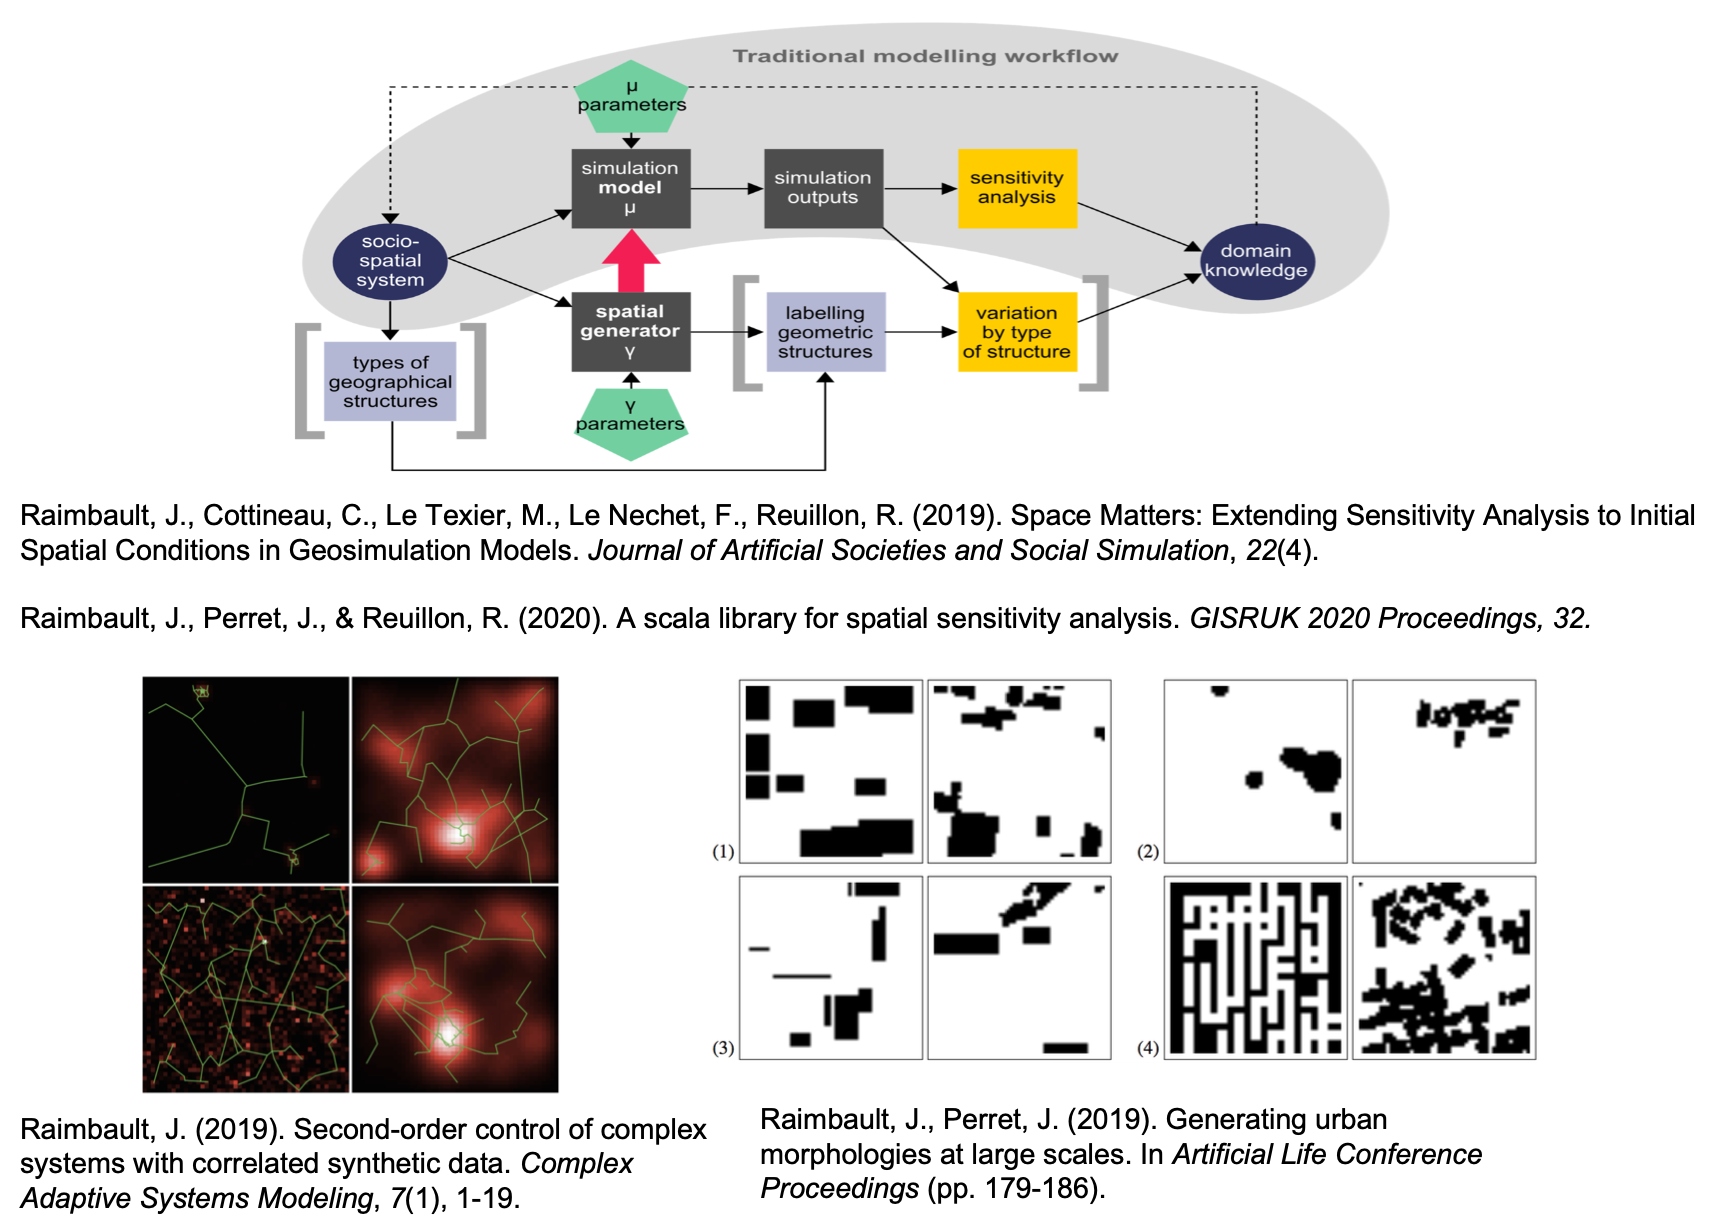
\includegraphics[width=0.95\linewidth]{figures/spatial_sa.png}

}





\section{OpenMOLE}

%To illustrate the reproducibility of our approach, we sketch the construction of the model with the OpenMOLE workflow engine, which provides a scripted workflow engine and methods to calibrate and validate simulation models, and suggest advanced numerical experiments for the validation of the coupled model.

\sframe{OpenMOLE workflow engine}{



OpenMOLE model exploration open source software \cite{reuillon2013openmole}

\medskip

\begin{center}

\includegraphics[height=0.13\textheight]{figures/iconOM.png}

\includegraphics[height=0.13\textheight]{figures/openmole.png}
\end{center}

\medskip

\textit{Enables seamlessly (i) model embedding; (ii) access to HPC resources; (iii) exploration and optimization algorithms}

\medskip

\url{https://openmole.org/}

}


\sframe{Towards advanced validation experiments}{

\textbf{OpenMOLE integrates methods for: } sensitivity analysis, spatial sensitivity analysis, design of experiments, calibration, diversity search, inverse problems, model reduction.

\bigskip

\begin{center}
	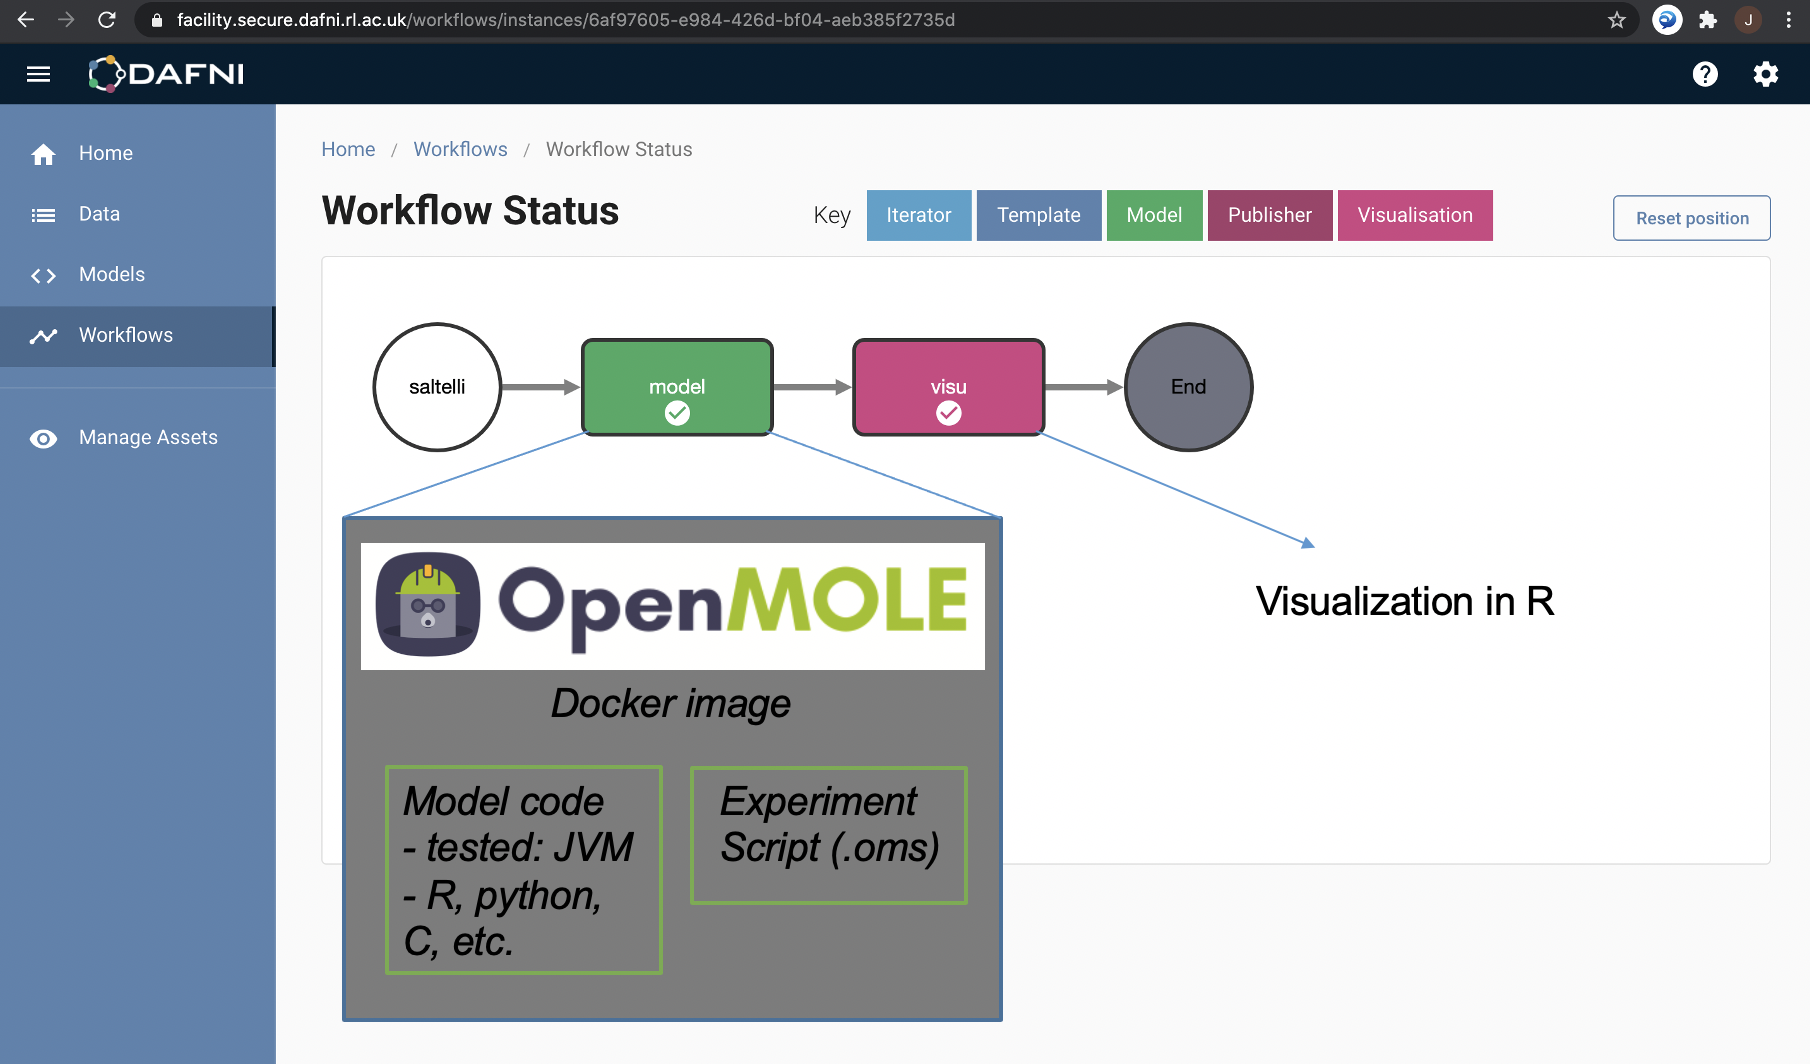
\includegraphics[width=0.75\linewidth]{figures/dafni-oml.png}
\end{center}

\textit{Integration of OpenMOLE into DAFNI}

}


\section{Discussion}

%We finally discuss ongoing developments on the application of this model to the development of health indicators within public transportation, and more particularly linking transportation and work-from-home policies with effective densities in public transport which provide potential exposure indicators in the context of the COVID-19 crisis.

\sframe{Discussion}{

\textbf{Developments}

\medskip

$\rightarrow$ Integration of multi-modal MATSim, calibration of mode choice parameters

\medskip

$\rightarrow$ Visualisation of MATSim agents dynamics (MATSim visu features not open)

\medskip

$\rightarrow$ Dynamical strong coupling of QUANT and SPENSER to combine population projections with the transport model

\bigskip

\textbf{Applications}

\medskip

$\rightarrow$ Validation of sub-models and integrated models using advanced model validation methods

\medskip

$\rightarrow$ Use MATSim outputs to quantify effective densities in public transport: potential exposure indicators in the COVID-19 context

\medskip

$\rightarrow$ Impact of policies and interventions on transport system dynamics and potential contaminations


}



\sframe{Conclusion}{


$\rightarrow$ Open, reproducible and validated urban models as elementary bricks towards larger integrated models


$\rightarrow$ Central role of the DAFNI platform: workflow system to couple models, data platform, integrated access to computational resources


\bigskip
\bigskip

\textbf{Open repositories}

\medskip

\url{https://github.com/JusteRaimbault/UrbanDynamics} for workflows

\medskip

\url{https://github.com/openmole/spatialdata} for data processing



\bigskip

\textbf{Workflow engines}

\medskip

DAFNI: \url{https://dafni.ac.uk/}

\medskip

OpenMOLE: \url{https://openmole.org}

}



%%%%%%%%%%%%%%%%%%%%%
\begin{frame}[allowframebreaks]
\frametitle{References}
\bibliographystyle{apalike}
\bibliography{biblio}
\end{frame}
%%%%%%%%%%%%%%%%%%%%%%%%%%%%




\end{document}

